
\section{Contexte historique}
\subsection{La ville de Douai au XIIIe siècle}

Douai trouve ses origines au VIe siècle sur un îlot de la Scarpe (\cite{mestayer_douai_2016}), une rivière traversant le nord de la France et se déversant dans le fleuve de l'Escaut. Les terres fertiles des alentours offrent une rapide croissance à ce qui n'est alors encore qu'une petite agglomération rurale. Dès le Xe siècle, l'agglomération s'étend sur les rives de la Scarpe. Au nord, sur la rive gauche de la rivière, le \textit{Duaculum}, appelé aussi le \textit{Douayeul}, une zone rurale dépendant de l'église Saint-Albin comprenant élevages de bêtes, greniers et brasseries (\cite{mestayer_douai_2016}). Sur l'autre rive, au sud, le \textit{Castel Bourgeois}, un quartier qui s'oriente davantage vers le commerce et l'artisanat. Ce dernier deviendra la première place marchande de la ville (\cite{netteghem_histoire_2021}). En 967, Douai, qui à cette époque est encore appelé \textit{Castrum Duacum}, se dote d'une place forte ainsi que d'une première muraille entourant la partie haute et basse de la ville (\cite{mestayer_douai_2016}). 

Forte de son activité agricole et de ses accès fluviaux, la ville gagne en richesse et devient un centre de commerce important dans la région qui attire marchands et artisans(\cite{clisant_vie_2003}). Les quartiers de la ville s'organisent alors en fonction des rassemblements d'artisans et marchands. On retrouve par exemple la rue des ferronniers, des foulons ou encore des bouchers. Les rues et places prennent à cette époque, où le pragmatisme  prévaut, une dénomination en fonction de leurs usages \cite{colin_decouvrez_2001}). 

Au XVIIe siècle, la disparité entre les deux rives se fait de plus en plus clivante et donne l'impression d'une ville séparée en deux entités distinctes (\cite{leroy-langelin_quartier_2012}). 
Le centre névralgique de la ville se consolide sur la rive droite de la Scarpe : une seconde enceinte, comportant douze portes, est édifiée afin d'englober l'expansion des quartiers autour du \textit{Castel bourgeois}, où des places de marchés ainsi que des halles apparaissent. 
Si le commerce céréalier fit démarrer la machine économique de la cité, Douai se forge maintenant une réputation, principalement, autour du commerce de draperies. Grâce aux foires de Champagne, la draperie douaisienne s'exporte à travers à toute l'Europe, et même au-delà (\cite{clisant_vie_2003}). Ce succès provient de la qualité et de la finition des étoffes produites, foulées aux pieds pour les plus précieuses. Chaque étape de la fabrication était supervisée par une des grandes familles bourgeoises de Douai (\cite{clisant_vie_2003}).
La progression économique que connait la ville grâce au commerce de draperies est très liée à la production agricole des campagnes avoisinantes, car ces dernières fournissent la matière première à cette nouvelle industrie.
Cependant, rapidement, la production de laine locale ne suffit plus à combler la demande en étoffes et un commerce s'installe avec l'Angleterre qui approvisionne alors Douai en laine(\cite{clisant_vie_2003}).

À la fin du XIIe siècle, un premier échevinage apparaît, constitué de douze riches et notables douaisiens (\cite{mestayer_douai_2016}. Ceux-ci régissent les activités, ainsi que les affaires financières, policières et juridiques de la ville au moyen de bans : une forme d'arrêté législatif (\cite{verriest_espinas_1914}). Ceci témoigne de la place, de plus en plus importante, qu'occupent les grandes familles bourgeoises dans l'administration et le développement de la ville.

Au cours de l'Histoire, Douai ne cesse d'être, tantôt française, tantôt flamande. Cependant, la richesse et la puissance de la ville font qu'elle garde toujours une certaine indépendance vis-à-vis du roi de France ou du comte de Flandre dans son administration (\cite{mestayer_douai_2016}).

La construction d'un nouveau rempart est entreprise au XIIIe siècle, justifié par l'apparition de nouveaux quartiers extérieurs à la seconde enceinte, tels que la \textit{Neuville} au  nord ou le \textit{Faubourg de Notre-Dame} à l'Est (\cite{netteghem_histoire_2021}).
Parallèlement à l'apogée économique de la ville, une nouvelle forme de marché\footnote{Ou de \og capitalisme \fg{} comme l'appelle G.Espinas (\fullcite{espinas_les_1933})} émerge : l'hiterage, qui recouvre toutes les formes de la propriété bâtie, y compris les terrains et les rentes de celles-ci. Ces bourgeois, principalement marchands et disposant déjà d'une certaine fortune mobilière, cherchent alors à acquérir biens-fonds et rentes ; un patrimoine qui devient un gage d'honorabilité et un signe de réussite dans la cité  (\cite{leguay_propriete_1989}). 

\begin{figure}[ht] % insère une figure ici (h = "here")
    \centering
    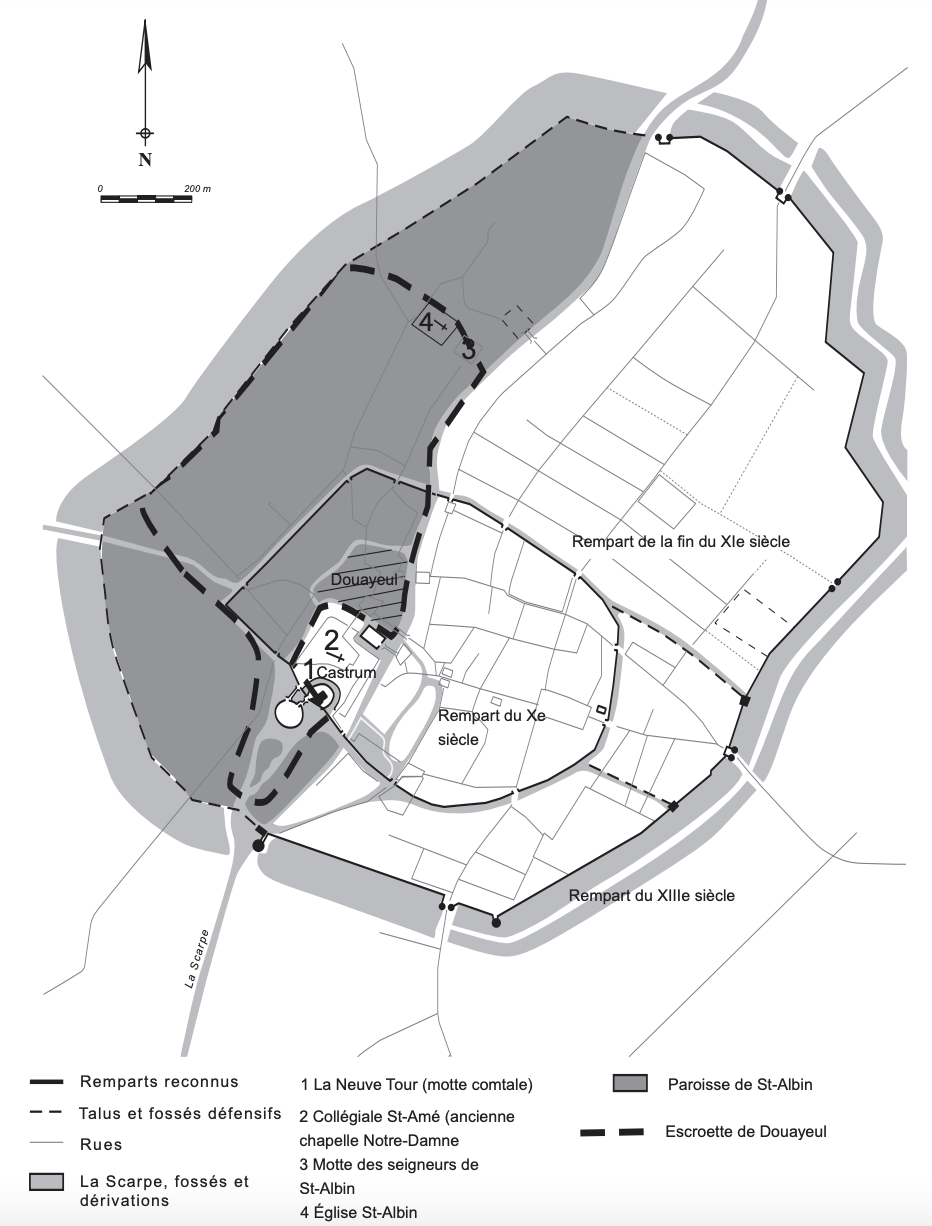
\includegraphics[scale=1]{1.Introduction/Img/Plan général de la ville de Douai avec les enceintes successives. DAO : E. Leroy-Langelin.png} 
    \caption{Plan général de Douai au XIIe s., E.Leroy-Langelin}
\end{figure}

\subsection{Sire Jean de France}
Sire Jean de France\footnote{On retrouve différentes graphies de cet anthroponyme, tel que \og Jehan de France\fg{} ou \og Jehans de Franche\fg{}, pour autant, il s'agit du même personnage. Cette pluralité de graphies des anthroponymes affecte également ses contemporains et sera traitée plus loin, dans le chapitre \textit{Méthodes}} est un bourgeois notable de Douai qui vécut dans la seconde moitié du XIIIe siècle. Il est, marchand drapier, propriétaire immobilier, à plusieurs reprises, échevin, par quelquefois, prêteur d'argent, notamment pour les comtes de Flandre, mais surtout patricien (\cite{espinas_les_1933}). 
Mais malgré ses titres à Douai et son patrimoine immobilier (estimé à 316 rentes sur 529 maisons , ainsi que quelques propriétés hors de la ville (\cite{blockmans_trois_1941})) on retrouve finalement assez peu de travaux de l'historiographie de ce personnage, resté dans l'ombre d'autres patriciens de Douai de la même époque.

Les dates de naissance et de mort de Jean de France ne sont pas connues avec exactitude, mais les premières traces de son existence remontent à 1252 et sa mort est supposée en 1298 (\cite{espinas_les_1933}). Nous savons qu'il avait comme mère Heluys, qui , par ailleurs, lui légua sa première rente\footfullcite[p.3]{espinas_les_1933}
On sait également qu'il  avait deux frères : Jakemes et Pieres et qu'il a eu au cours de sa vie, une fille, Hielotain, qui devint abbesse du monastère de Sin-le-Noble. En revanche, il n'a été retrouvé aucune mention de son père (\cite{espinas_les_1933}).

Le régime patricien, fut caractérisé par une exploitation de la misère, principalement celle des ouvriers et des universitaires (\cite{blockmans_trois_1941}). La figure la plus emblématique de patriciat est sans doute Jehan Boinebroke  que Fr. Blockmans nous décrit comme tel :
\begin{displayquote} 
    \og J. Boinebroke apparaît comme l'incarnation d'un capitalisme tellement hideux, si cruel et si impitoyable, que même la première moitié du xixe siècle n'en a pas connu de pareil ! \fg{}\footfullcite[p. 266]{blockmans_trois_1941}
\end{displayquote}
\vspace{0,5cm}
À son opposition, Jean de France est dépeint par G. Espinas et Fr. Blockmans comme un investisseur prudent et plutôt bienveillant :
\begin{displayquote}
    \og [...] il représente d’une façon directe une forme de capitalisme foncier sortie de la propriété immobilière. Cependant, ce n’est pas un égoïste..Il a pu jouir de son argent, de ses revenus pour lui-même, mais il ne les a pas gardés exclusivement pour lui, il a pensé aux malheureux, aux « déshérités de la vie » et sans doute, mù expressément par une pensée religieuse, il a fondé en leur faveur une institution de bienfaisance : il s’est montré un riche charitable.\fg{} 
    \footfullcite[p.139]{espinas_les_1933} 
\end{displayquote} 
\vspace{0,5cm}
D'ailleurs, lors des insurrections du peuple antipatriciennes qui frappèrent Douai à la fin du XIIIe siècle, le nom de Jean de France ne figura pas sur la liste des bannis malgré son appartenance indéniable à l'élite bourgeoise de la ville(\cite{espinas_les_1933}).

\subsection{Registre de rentes de Jean de France}
Le registre de rente de Jean de France, ou pour reprendre du document même, \textit{l'escris}, est un document d'origine privé, écrit en picard médiévale, déposé à l'hospice des Chartriers de Douai en octobre 1291. 

Le document recense toutes les rentes de Sire Jean de France à la date du dépôt (octobre 1291). Celles-ci sont classées par ordre topographique selon les \textit{escroetes} (\cite{espinas_les_1933}). Les \textit{escroetes} sont au nombre de six et divisent la ville en quartiers. Elles sont : \textit{li escroete dou Markiet}, \textit{li escroete de Canteleu}, \textit{li escroete dou Més}, \textit{li escroette des Wés}, \textit{li escroete de Douayeul}, \textit{li escroete de Neuville}.
Ces \textit{escroetes}, sont elles-mêmes divisées en sous-éléments topographiques correspondant la plupart du temps aux connétablies. Il peut s'agir de rues, de places, de porte, etc. Finalement, s'il s'agit de rues ou de places importantes, ces subdivisions sont encore une fois divisées en fonction du \textit{rench}, correspondant au rang de la voie.

De par sa complétude et son écriture, qui ne comporte que très peu d'imperfections et d'irrégularités, cet ouvrage est particulièrement précieux pour approcher le contexte économique et social de l'époque. 
Toutefois, il faut pouvoir appréhender cette source de la manière dont il conviens : certains éléments sont obscures ou donne lieu à des interrogations. Pour cause, il s'agit là d'un document de résultats et non de formation (\cite{espinas_les_1933}).

L'utilisation du registre prend toute sa pertinence dans nos recherches, car chaque entrée contient, non seulement le nom du débirentier
%\footnote{\og Personne qui doit une rente.\fg{} définition du dictionnaire Larousse, consulté à la date du 26/09/2022 https://www.larousse.fr/dictionnaires/francais/d\%C3\%A9birentier/21806} 
et le montant, ainsi que le type de la rente, mais également une indication sur la localisation de la propriété. Cependant, cette information est donnée de manière indirecte en citant le nom des habitants des propriétés voisines, ou dans de rares cas, les éléments topographiques adjacents comme une porte (d'enceinte), une place ou une chapelle.